\begin{figure}
\centering
\begin{subfigure}{0.3\textwidth}
\centering
\begin{tikzpicture}[declare function={f(\x)=2-1/9*\x^2;}]
\pgfmathsetmacro{\ka}{0.75}
\pgfmathsetmacro{\kb}{3}
\pgfmathsetmacro{\kc}{2.2}
\pgfmathsetmacro{\kd}{2.5}
\pgfmathsetmacro{\ra}{f(\ka)}
\pgfmathsetmacro{\rb}{f(\kb)}
\pgfmathsetmacro{\rc}{f(\kc)}
\pgfmathsetmacro{\rd}{f(\kd)}
\draw(-0.25,0)--(\ka-1/4*\ra,0);
\draw[-latex](\kb-1/4*\rb,0)--(3.5,0)node[right]{$x$};
\draw[-latex](0,-0.2)--(0,2.2)node[above]{$y$};
\draw[]plot[domain=\ka:\kb](\x,{f(\x)});
\draw[very thick]plot[domain=\kc:\kd](\x,{f(\x)});
\draw[]plot[domain=\ka:\kb](\x,{-f(\x)});
\draw(\kb,0) circle (1/4*\rb cm and \rb cm);
\draw([shift={(90:1/4*\ra cm and \ra cm)}]\ka,0) arc (90:270:1/4*\ra cm and \ra cm);
\draw([shift={(90:1/4*\rc cm and \rc cm)}]\kc,0) arc (90:270:1/4*\rc cm and \rc cm);
\draw([shift={(90:1/4*\rd cm and \rd cm)}]\kd,0) arc (90:270:1/4*\rd cm and \rd cm);
\draw[gray](\ka,0)node[circ]{}node[below]{$a$};
\draw(\kb,0)node[circ]{}node[below]{$b$};
\draw(\kc,{f(\kc)})node[above]{$P$};
\draw(\kd,{f(\kd)})node[above,xshift=1mm]{$Q$};
\draw(\ka,{f(\ka)})node[above right]{$y=f(x)$};
\end{tikzpicture}
\caption{}
\end{subfigure}\hfill
\begin{subfigure}{0.3\textwidth}
\centering
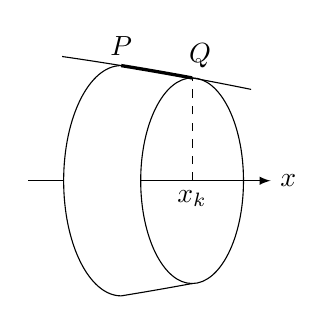
\begin{tikzpicture}[xscale=3,declare function={f(\x)=2-1/9*\x^2;}]
\pgfmathsetmacro{\ka}{0.75}
\pgfmathsetmacro{\kb}{3}
\pgfmathsetmacro{\kc}{2.2}
\pgfmathsetmacro{\kd}{2.5}
\pgfmathsetmacro{\ra}{f(\ka)}
\pgfmathsetmacro{\rb}{f(\kb)}
\pgfmathsetmacro{\rc}{f(\kc)}
\pgfmathsetmacro{\rd}{f(\kd)}
\draw(-1/6*\rc,0)--++(-0.15,0);
\draw[-latex](\kd-\kc-1/6*\rd,0)--++(0.55,0)node[right]{$x$};
\draw[very thick]plot[domain=\kc:\kd](\x-\kc,{f(\x)});
\draw[]plot[domain=\kc-0.25:\kd+0.25](\x-\kc,{f(\x)});
\draw[]plot[domain=\kc:\kd](\x-\kc,{-f(\x)});
\draw([shift={(90:1/6*\rc cm and \rc cm)}]0,0) arc (90:270:1/6*\rc cm and \rc cm);
\draw(\kd-\kc,0) circle (1/6*\rd cm and \rd cm);
\draw(0,{f(\kc)})node[above]{$P$};
\draw(\kd-\kc,{f(\kd)})node[above,xshift=1mm]{$Q$};
\draw[dashed](\kd-\kc,0)node[below]{$x_k$}--++(0,{f(\kd)});
\end{tikzpicture}
\caption{}
\end{subfigure}\hfill
\begin{subfigure}{0.3\textwidth}
\centering
\begin{tikzpicture}[xscale=0.5,yscale=1.5,declare function={f(\x)=1-1/4*\x;}]
\pgfmathsetmacro{\ka}{0}
\pgfmathsetmacro{\kb}{1.5}
\pgfmathsetmacro{\ra}{f(\ka)}
\pgfmathsetmacro{\rb}{f(\kb)}
\draw[dashed](-0.5,0)--(\kb-1/4*\rb,0);
\draw[-latex](\kb-1/4*\rb,0)--(5,0)node[right]{$x$};
\draw[]plot[domain=0:\kb](\x,{f(\x)});
\draw[]plot[domain=0:\kb](\x,{-f(\x)});
\draw[dashed]plot[domain=\kb:4](\x,{f(\x)});
\draw[dashed]plot[domain=\kb:4](\x,{-f(\x)});
\draw([shift={(90:1/2*\ra cm and \ra cm)}]\ka,0) arc (90:270:1/2*\ra cm and \ra cm);
\draw(\kb,0) circle (1/2*\rb cm and \rb cm);
\draw(0,0)--(0,{f(0)})node[pos=0.5,right]{$r_1$};
\draw(\kb,0)--(\kb,{f(\kb)})node[pos=0.4,right,fill=white]{$r_2$};
\draw[stealth-stealth](0,{f(0)+0.1})--(\kb,{f(\kb)+0.1})node[pos=0.25,above right]{\RL{ترچھی لمبائی $L$}};
\end{tikzpicture}
\caption{}
\end{subfigure}
\end{figure}

\begin{figure}
\centering
\begin{minipage}{0.45\textwidth}
\centering
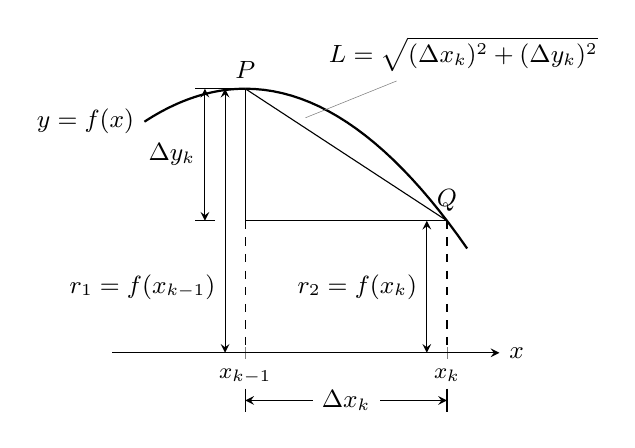
\begin{tikzpicture}[font=\small,declare function={f(\x)=2-\x^2;}]
\begin{axis}[clip=false,small,axis lines=middle,axis y line=none,ymin=0,xtick={\a,\c},xticklabels={$x_{k-1}$,$x_k$},enlargelimits=true,xlabel={$x$},xlabel style={at={(current axis.right of origin)},anchor=west}]
\pgfmathsetmacro{\a}{0}
\pgfmathsetmacro{\b}{1.1}
\pgfmathsetmacro{\c}{1}
\addplot[thick,domain=0:\b]{f(x)};
\addplot[thick,domain=0:0.5]({-x},{f(x)})node[pos=1,left]{$y=f(x)$};
\draw(\a,{f(\a)})node[above]{$P$}--(\c,{f(\c)})node[above]{$Q$}node[pos=0.25,pin=60:{$L=\sqrt{(\Delta x_k)^2+(\Delta y_k)^2}$}]{};
\draw[dashed](0,{f(\c)})--(0,0);
\draw[dashed](\c,{f(\c)})--(\c,0);
\draw(\c,{f(\c)})--(0,{f(\c)})--(0,{f(0)});
\RightAngle{(\c,{f(\c)})}{(0,{f(\c)})}{(0,{f(0)})}
\draw[stealth-stealth](\c-0.1,0)--(\c-0.1,{f(\c)})node[pos=0.5,left]{$r_2=f(x_k)$};
\draw[stealth-stealth](-0.1,0)--(-0.1,{f(0)})node[pos=0.25,left]{$r_1=f(x_{k-1})$};
\draw[stealth-stealth](-0.2,{f(\c)})--(-0.2,{f(0)})node[pos=0.5,left]{$\Delta y_k$};
\draw(-0.15,{f(\c)})--(-0.25,{f(\c)});
\draw(-0.05,{f(0)})--(-0.25,{f(0)});
\draw[stealth-stealth](0,-4ex)--(\c,-4ex)node[pos=0.5,fill=white]{$\Delta x_k$};
\draw(0,-3ex)--(0,-5ex);
\draw(\c,-3ex)--(\c,-5ex);
\end{axis}
\end{tikzpicture}
\caption{قطع $PQ$ کی لمبائی کے ساتھ وابستہ متغیرات۔}
\end{minipage}\hfill
\begin{minipage}{0.45\textwidth}
\centering
\begin{tikzpicture}[font=\small,declare function={f(\x)=2-\x^2;g(\x)=7/4-(\x-1/2);}]
\begin{axis}[clip=false,small,axis lines=middle,axis y line=none,ymin=0,xtick={\a,\c,0.5},xticklabels={$x_{k-1}$,$x_k$,$c_k$},enlargelimits=true,xlabel={$x$},xlabel style={at={(current axis.right of origin)},anchor=west}]
\pgfmathsetmacro{\a}{0}
\pgfmathsetmacro{\b}{1.1}
\pgfmathsetmacro{\c}{1}
\addplot[thick,domain=0:\b]{f(x)};
\addplot[thick,domain=0:0.5]({-x},{f(x)})node[pos=1,left]{$y=f(x)$};
\addplot[domain=-0.1:\b]{g(x)};
\draw(\a,{f(\a)})node[above left]{$P$}--(\c,{f(\c)})node[right]{$Q$};
\draw[dashed](0,{f(\c)})--(0,0);
\draw[dashed](\c,{f(\c)})--(\c,0);
\draw(\c,{f(\c)})--(0,{f(\c)})--(0,{f(0)});
\RightAngle{(\c,{f(\c)})}{(0,{f(\c)})}{(0,{f(0)})}
\draw[stealth-stealth](-0.2,{f(\c)})--(-0.2,{f(0)})node[pos=0.5,left]{$\Delta y_k$};
\draw(-0.15,{f(\c)})--(-0.25,{f(\c)});
\draw(-0.15,{f(0)})--(-0.25,{f(0)});
\draw[stealth-stealth](0,-4ex)--(\c,-4ex)node[pos=0.5,fill=white]{$\Delta x_k$};
\draw(0,-3ex)--(0,-5ex);
\draw(\c,-3ex)--(\c,-5ex);
\draw(1/2,{f(1/2)})node[circ]{}node[above right]{$(c_k,f(c_k))$}--(1/2,0);
\end{axis}
\end{tikzpicture}
\caption{خط مستقیم $PQ$ اور نقطہ $c_k$ پر مماس متوازی ہیں۔}
\end{minipage}\hfill
\end{figure}

\begin{figure}
\centering
\begin{minipage}{0.45\textwidth}
\centering
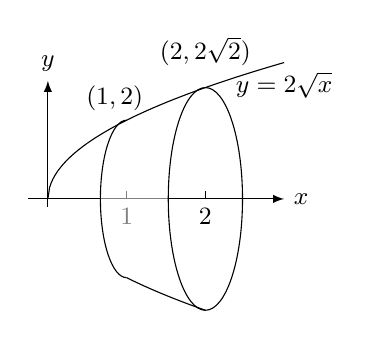
\begin{tikzpicture}[font=\small,yscale=0.5,declare function={f(\x)=2*sqrt(\x);}]
\pgfmathsetmacro{\a}{1}
\pgfmathsetmacro{\b}{2}
\pgfmathsetmacro{\ra}{f(\a)}
\pgfmathsetmacro{\rb}{f(\b)}
\draw(\a-1/6*\ra,0)--(-0.25,0);
\draw[gray](\a-1/6*\ra,0)--(\b-1/6*\rb,0);
\draw[-latex](\b-1/6*\rb,0)--(3,0)node[right]{$x$};
\draw[-latex](0,-0.2)--(0,3)node[above]{$y$};
\draw[]plot[domain=0:0.5](\x,{f(\x)});
\draw[]plot[domain=0.5:3](\x,{f(\x)});
\draw[]plot[domain=1:2](\x,{-f(\x)});
\draw([shift={(90:1/6*\ra cm and \ra cm)}]\a,0) arc (90:270:1/6*\ra cm and \ra cm);
\draw(\b,0) circle (1/6*\rb cm and \rb cm);
\draw(\a,{f(\a)})node[above,xshift=-1ex]{$(1,2)$};
\draw(\b,{f(\b)})node[above,yshift=1ex]{$(2,2\sqrt{2})$};
\draw(3,{f(3)})node[below]{$y=2\sqrt{x}$};
\draw(2,0)node[below]{$2$}--(2,0.2);
\draw[gray](1,0)node[below]{$1$}--(1,0.2);
\end{tikzpicture}
\end{minipage}\hfill
\begin{minipage}{0.45\textwidth}
\centering
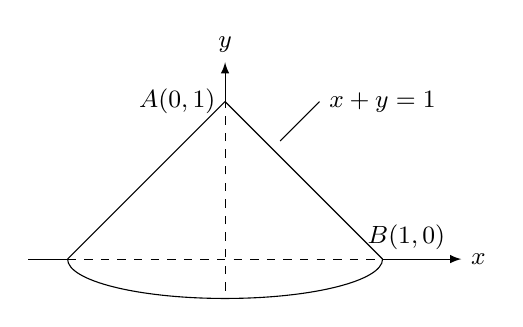
\begin{tikzpicture}[scale=2,font=\small,declare function={f(\x)=1-\x;}]
\draw[dashed](-1,0)--(1,0);
\draw(-1,0)--(-1.25,0);
\draw[-latex](1,0)node[above,xshift=2ex]{$B(1,0)$}--(1.5,0)node[right]{$x$};
\draw[dashed](0,-0.2)--(0,1)node[left]{$A(0,1)$};
\draw[-latex](0,1)--(0,1.25)node[above]{$y$};
\draw[]plot[domain=0:1](\x,{f(\x)});
\draw[]plot[domain=0:1](-\x,{f(\x)});
\draw([shift={(180:1cm and 0.25 cm)}]0,0) arc (180:360:1cm and 0.25 cm);
\draw(0.25,{f(0.25)})++(0.1,0)--++(0.25,0.25)node[right]{$x+y=1$};
\end{tikzpicture}
\end{minipage}\hfill
\end{figure}


\begin{figure}
\centering
\begin{minipage}{0.45\textwidth}
\centering
\begin{tikzpicture}[font=\small,declare function={f(\x)=(\x-1)*(\x-1.75)*(\x-2.5)+1;}]
\pgfmathsetmacro{\a}{0.75}
\pgfmathsetmacro{\b}{2.5}
\pgfmathsetmacro{\c}{1.8}
\pgfmathsetmacro{\d}{2}
\pgfmathsetmacro{\e}{1/2*(\c+\d)}
\pgfmathsetmacro{\ra}{f(\a)}
\pgfmathsetmacro{\rb}{f(\b)}
\pgfmathsetmacro{\rc}{f(\c)}
\pgfmathsetmacro{\rd}{f(\d)}
\draw[-latex](0,-0.2)--(0,1.5);
\draw[-latex](-0.25,0)--(3.5,0)node[right]{\RL{محور طواف}};
\draw[thick]plot[domain=0.75:2.5](\x,{f(\x)});
\draw[]plot[domain=0.75:2.5](\x,{-f(\x)});
\draw([shift={(90:1/4*\ra cm and \ra cm)}]\a,0) arc (90:270:1/4*\ra cm and \ra cm);
\draw(\b,0) circle (1/4*\rb cm and \rb cm);
\draw([shift={(90:1/4*\rc cm and \rc cm)}]\c,0) arc (90:270:1/4*\rc cm and \rc cm);
\draw([shift={(90:1/4*\rd cm and \rd cm)}]\d,0) arc (90:270:1/4*\rd cm and \rd cm);
\draw(\a,{f(\a)})node[left]{$A$};
\draw(\b,{f(\b)})node[right]{$B$};
\draw(\b,0)node[below]{$b$}--(\b,{f(\b)});
\draw[gray](\a,0)node[below]{$a$}--(\a,{f(\a)});
\draw[gray](\e,0)--(\e,{f(\e)})node[pos=0.5,right]{$\rho$};
\draw(\c,{f(\c)+0.1})--++(0,0.2)coordinate[pos=0.5](L);
\draw(\d,{f(\c)+0.1})--++(0,0.2)coordinate[pos=0.5](R);
\draw[stealth-](L)--++(-0.2,0);
\draw[stealth-](R)--++(0.3,0)--++(0,0.2)node[above]{$\dif s$};
\draw(\b+0.25,{f(\c)+0.5})node[right]{$S=\int\limits_a^b2\pi \rho \dif s$};
\end{tikzpicture}
\end{minipage}\hfill
\begin{minipage}{0.45\textwidth}
\centering
\begin{tikzpicture}[xscale=4,yscale=10,font=\small,declare function={f(\x)=\x^3;}]
\pgfmathsetmacro{\a}{1/2}
\pgfmathsetmacro{\ra}{f(\a)}
\draw[-latex](0,-0.15)--(0,0.175)node[above]{$y$};
\draw[]plot[domain=0:\a](\x,{f(\x)});
\draw[]plot[domain=0:\a](\x,{-f(\x)});
\draw(\a,0) circle (1/3*\ra cm and \ra cm);
\draw[-latex](\a-1/3*\ra,0)--(0.7,0)node[right]{$x$};
\draw(\a,0)node[below]{$\tfrac{1}{2}$}--++(0,0.01);
\draw(0.35,{f(0.35)})node[above left]{$y=x^3$};
\draw(\a,{f(\a)})node[above]{$\big(\tfrac{1}{2},\tfrac{1}{8}\big)$};
\draw(0,\ra)node[left]{$\tfrac{1}{8}$}--++(0.01,0);
\draw(0,-\ra)node[left]{$-\tfrac{1}{8}$}--++(0.01,0);
\end{tikzpicture}
\end{minipage}
\end{figure}
